\section{Mesh properties} \label{app:appMesh}

    \renewcommand{\thepage}{\arabic{page}}
    \setcounter{page}{\thelastPage}

\subsection{Non orthogonality} \label{sec:nonOrtho}
    The non orthogonality is a mesh \textbf{property} (Figure~\ref{fig:nonOrtho}) based on the \textit{vectorial} difference between the face normal versor $\boldsymbol{n}$ - at face middle point $P$ - and the versor between the control volume and its neighbour cell, $\overline{C_1 C_2}$. This property is expressed through $\theta_{no}$: the closer to $0$ the better. The non orthogonality importance is related to the \verb|FVM| that bases the fluxes computation on vector $\boldsymbol{n}$. 

\definecolor{qqwuqq}{rgb}{0,0.39,0}
\definecolor{ffqqqq}{rgb}{1,0,0}
\definecolor{qqqqff}{rgb}{0,0,1}
\definecolor{qqttff}{rgb}{0,0.2,1}
\definecolor{zzttqq}{rgb}{0.6,0.2,0}
\definecolor{cqcqcq}{rgb}{0.75,0.75,0.75}
\begin{figure}[h!]
    \centering
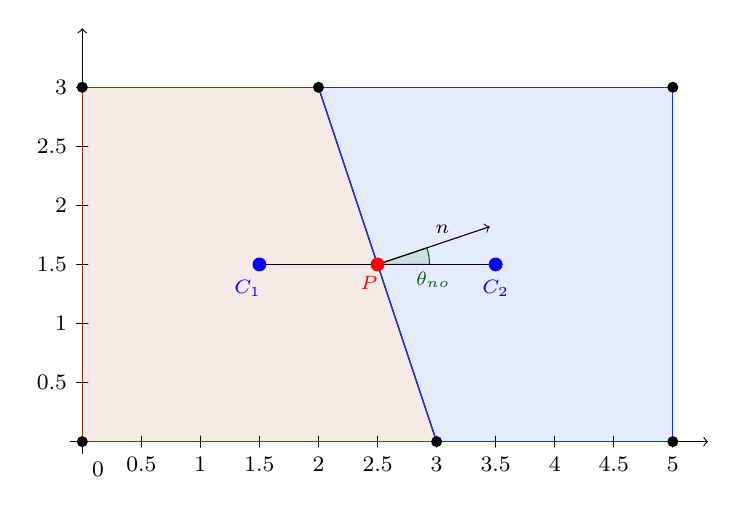
\begin{tikzpicture}[line cap=round,line join=round,x=1.5cm,y=1.5cm]
%\draw [color=cqcqcq,dash pattern=on 1pt off 1pt, xstep=0.5cm,ystep=0.5cm] (-0.1,-0.1) grid (5.3,3.5);
\draw[->,color=black] (-0.1,0) -- (5.3,0);
\foreach \x in {,0.5,1,1.5,2,2.5,3,3.5,4,4.5,5}
\draw[shift={(\x,0)},color=black] (0pt,2pt) -- (0pt,-2pt) node[below] {\footnotesize $\x$};
\draw[->,color=black] (0,-0.1) -- (0,3.5);
\foreach \y in {,0.5,1,1.5,2,2.5,3}
\draw[shift={(0,\y)},color=black] (2pt,0pt) -- (-2pt,0pt) node[left] {\footnotesize $\y$};
\draw[color=black] (0pt,-10pt) node[right] {\footnotesize $0$};
\clip(-0.1,-0.1) rectangle (5.3,3.5);
\fill[color=zzttqq,fill=zzttqq,fill opacity=0.1] (0,3) -- (0,0) -- (3,0) -- (2,3) -- cycle;
\fill[color=qqttff,fill=qqttff,fill opacity=0.1] (2,3) -- (3,0) -- (5,0) -- (5,3) -- cycle;
\draw [shift={(2.5,1.5)},color=qqwuqq,fill=qqwuqq,fill opacity=0.1] (0,0) -- (0:0.44) arc (0:18.43:0.44) -- cycle;
\draw (0,3)-- (0,0);
\draw (3,0)-- (0,0);
\draw (3,0)-- (2,3);
\draw (2,3)-- (0,3);
\draw (2,3)-- (5,3);
\draw (5,3)-- (5,0);
\draw (3,0)-- (5,0);
\draw [color=zzttqq] (0,3)-- (0,0);
\draw [color=zzttqq] (0,0)-- (3,0);
\draw [color=zzttqq] (3,0)-- (2,3);
\draw [color=zzttqq] (2,3)-- (0,3);
\draw [color=qqttff] (2,3)-- (3,0);
\draw [color=qqttff] (3,0)-- (5,0);
\draw [color=qqttff] (5,0)-- (5,3);
\draw [color=qqttff] (5,3)-- (2,3);
\draw (1.5,1.5)-- (3.5,1.5);
\draw [->] (2.5,1.5) -- (3.45,1.82);
\begin{scriptsize}
\fill [color=black] (0,3) circle (2.0pt);
\fill [color=black] (0,0) circle (2.0pt);
\fill [color=black] (3,0) circle (2.0pt);
\fill [color=black] (2,3) circle (2.0pt);
\fill [color=black] (5,3) circle (2.0pt);
\fill [color=black] (5,0) circle (2.0pt);
\fill [color=qqqqff] (1.5,1.5) circle (2.5pt);
\draw[color=qqqqff] (1.4,1.3) node {$C_1$};
\fill [color=qqqqff] (3.5,1.5) circle (2.5pt);
\draw[color=qqqqff] (3.5,1.3) node {$C_2$};
\fill [color=ffqqqq] (2.5,1.5) circle (2.5pt);
\draw[color=ffqqqq] (2.43,1.34) node {$P$};
\draw[color=black] (3.05,1.8) node {$n$};
\draw[color=qqwuqq] (2.97,1.37) node {$\theta_{no}$};
\end{scriptsize}
\end{tikzpicture}
    \caption{Non orthogonality.}
    \label{fig:nonOrtho}
\end{figure}


There are many correctors for this topologic issue that are related on flux corrections. One of the main numeric operator that suffers a lot of bad non orthogonality values is the laplacian, $\boldsymbol{\Delta}$. One of the most important equation related to $\boldsymbol{\Delta}$ is the \textbf{Helmolts} equation - \textbf{Poisson} equation in the incompressible cases - that is about mass conservation (one of the most important principles to satisfy). Good non orthogonality values (in OpenFOAM syntax) are: $75 - 80$.

\subsection{Skewness} \label{sec:skewness}
As the non orthogonality, the skewness is a mesh \textbf{property} (Figure~\ref{fig:skewness}). This property is extremelly dependent on mesh topology and it has a very important effect on the simulation. This property is based on the computation of a quantity at face center. To compute this quantity, the \verb|FVM| uses an interpolatory scheme that is based on control volumes' center distances. If the approximation of the field - and then the interpolation of fluxes at face center based on this field - is wrong, the whole simulation will suffer of sources/sinks like presence in the domain that will bring to errors in the results and also to having bad effects on covergence rates. 
    
\begin{figure}[h!]
    \centering
\begin{tikzpicture}[line cap=round,line join=round,x=2cm,y=2cm]
%\draw [color=cqcqcq,dash pattern=on 1pt off 1pt, xstep=1.5cm,ystep=1.5cm] (-0.1,-0.1) grid (3.7,2.2);
\draw[->,color=black] (-0.1,0) -- (3.7,0);
\foreach \x in {,1,2,3}
\draw[shift={(\x,0)},color=black] (0pt,2pt) -- (0pt,-2pt) node[below] {\footnotesize $\x$};
\draw[->,color=black] (0,-0.1) -- (0,2.2);
\foreach \y in {,1,2}
\draw[shift={(0,\y)},color=black] (2pt,0pt) -- (-2pt,0pt) node[left] {\footnotesize $\y$};
\draw[color=black] (0pt,-10pt) node[right] {\footnotesize $0$};
\clip(-0.1,-0.1) rectangle (3.7,2.2);
\fill[color=zzttqq,fill=zzttqq,fill opacity=0.1] (0.5,2) -- (0,0) -- (2,0.5) -- (2.5,2) -- cycle;
\fill[color=ttttff,fill=ttttff,fill opacity=0.1] (2,0.5) -- (3.5,0) -- (3.5,1.5) -- (2.5,2) -- cycle;
\draw (0.5,2)-- (0,0);
\draw (0,0)-- (2,0.5);
\draw (2,0.5)-- (3.5,0);
\draw (3.5,0)-- (3.5,1.5);
\draw (0.5,2)-- (2.5,2);
\draw (2.5,2)-- (3.5,1.5);
\draw (2.5,2)-- (2,0.5);
\draw [color=zzttqq] (0.5,2)-- (0,0);
\draw [color=zzttqq] (0,0)-- (2,0.5);
\draw [color=zzttqq] (2,0.5)-- (2.5,2);
\draw [color=zzttqq] (2.5,2)-- (0.5,2);
\draw [color=ttttff] (2,0.5)-- (3.5,0);
\draw [color=ttttff] (3.5,0)-- (3.5,1.5);
\draw [color=ttttff] (3.5,1.5)-- (2.5,2);
\draw [color=ttttff] (2.5,2)-- (2,0.5);
\draw [line width=2pt] (1.39,1.11)-- (2.94,1.13);
\draw [line width=2pt] (1.39,1.11)-- (2.25,1.25);
\draw [line width=2pt] (2.25,1.25)-- (2.94,1.13);
\begin{scriptsize}
\fill [color=black] (0.5,2) circle (2.0pt);
\fill [color=black] (0,0) circle (2.0pt);
\fill [color=black] (2,0.5) circle (2.0pt);
\fill [color=black] (2.5,2) circle (2.0pt);
\fill [color=black] (3.5,0) circle (2.0pt);
\fill [color=black] (3.5,1.5) circle (2.0pt);
\fill [color=ffqqqq] (2.25,1.25) circle (2.5pt);
\draw[color=ffqqqq] (2.19,1.5) node {$P$};
\fill [color=ttttff] (1.39,1.11) circle (2.5pt);
\draw[color=ttttff] (1.16,1.02) node {$C_1$};
\fill [color=ttttff] (2.94,1.13) circle (2.5pt);
\draw[color=ttttff] (3.19,1.02) node {$C_2$};
\draw[color=black] (1.91,0.92) node {$d$};
\draw[color=black] (1.91,1.38) node {$d_1$};
\draw[color=black] (2.68,1.37) node {$d_2$};
\end{scriptsize}
\end{tikzpicture}
    \caption{Skewness.}
    \label{fig:skewness}
\end{figure}


In contrast to the non orthogonality property, this property cannot be numerically \textbf{fixed}. As consequence, it is necessary to have meshes with the lowest skewness possible. It can happen that bad skewness brings to remeshing all the domain. Good skewness values (in OpenFOAM syntax) are: $1 - 8$. 
